\subsubsection{Beam Search}
Before understanding the PICARD, let us first understand the concept of Beam Search:

\begin{figure}[H]
    \centering
    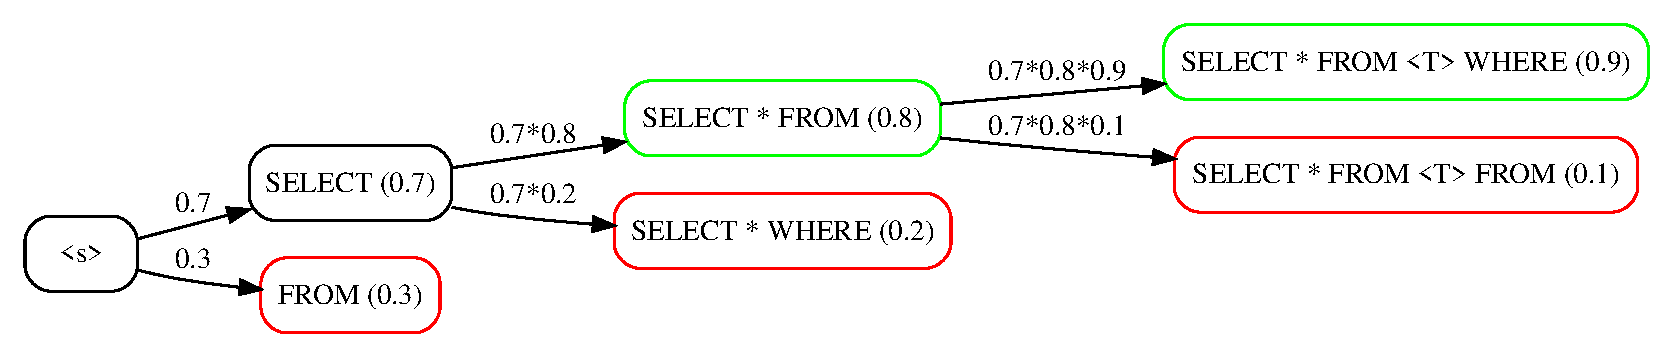
\includegraphics[width=0.8\textwidth]{pics/picard/beam/beam.eps}
    \caption{2-Beam Search}
    \label{fig:beam_search}
\end{figure}

Beam search is a widely used search algorithm in natural language processing and machine learning. It is beneficial in sequence-to-sequence (seq2seq) models, which generate output sequences based on input sequences. Beam search is used to find the most likely sequence of output words given an input sequence.
\\
The basic idea behind beam search is to maintain a set of the most likely sequences at each step of the decoding process. This set of sequences called the "beam," is initially set to the starting point of the decoding process, and at each step, new sequences are generated by considering all the following possible words. The new sequences are then ranked based on their likelihood, and the highest-ranking sequences are added to the beam. The process is repeated until a stopping criterion is met \cite{10.1371/journal.pone.0211558}.
Beam search is handy in seq2seq models because it allows the model to generate multiple output sequences rather than just a single sequence. This is important because, in many cases, there may be multiple valid outputs for a given input sequence. By generating multiple outputs, beam search allows the model to explore the space of possible outputs and find the most likely sequences.
\\
One of the critical advantages of beam search is that it is computationally efficient. Because it only considers a small number of sequences at each step, it can quickly find the most likely sequences without exploring the entire space of possible outputs. This makes it well-suited for use in applications with limited computational resources, such as on mobile devices or in real-time systems.
Another advantage of beam search is that it can be used with other techniques, such as attention mechanisms, to improve the performance of seq2seq models. Attention mechanisms allow the model to focus on specific parts of the input sequence when generating the output, which can help to improve the quality of the generated sequences.
\\
In conclusion, Beam Search is a robust algorithm widely used in natural language processing and machine learning, particularly in the context of sequence-to-sequence (seq2seq) models. It allows the model to generate multiple output sequences rather than just a single sequence and is computationally efficient, making it well-suited for use in applications where computational resources are limited. Additionally, it can be combined with other techniques, such as attention mechanisms, to improve the performance of seq2seq models.